%%%
%%% Document class and page properties
%%%

\documentclass{IIBproject}

% Set margin size
\usepackage[margin=2.5cm]{geometry}

% Set table of contents depth
\setcounter{tocdepth}{2}

%%%
%%% Standard packages in alphabetical order
%%%

% Use the AMS math package for special fonts such as mathbb (included in the amssymb package
% coming with ams math), inline text in equations, etc.
\usepackage{amsmath}
\usepackage{amssymb}

% Use the calc package for infix arithmetic
\usepackage{calc}

% Use BibTeX for bibliography management, use the hyperref package to include URLs in the entries
\usepackage{cite}
\usepackage{url}

% Color text
\usepackage{color}

% Use the package for declaring paired delimiters
\usepackage{mathtools}

% Sets 1.5 line spacing
\usepackage{setspace}
\onehalfspacing

% Provides formatting of numbers (here used for thousands' separators)
\usepackage{siunitx}

% Use the tikz package for drawing
\usepackage{tikz}

\usetikzlibrary{decorations.pathreplacing}

% Provides robust spaces after commands
\usepackage{xspace}

%%%
%%% Commands
%%%

% Declare paired delimiters
\DeclarePairedDelimiter{\ceil}{\lceil}{\rceil}
\DeclarePairedDelimiter{\bracket}{(}{)}

% Define macros for correct spacing after abbreviations, source: http://tex.stackexchange.com/a/15017
\newcommand*{\eg}{e.g.\@\xspace}
\newcommand*{\ie}{i.e.\@\xspace}

% Abbreviations which can occur at the end of the sentence cannot duplicate the following dot
\makeatletter
\DeclareRobustCommand*{\AbbreviationWithDot}[1]{\@ifnextchar{.}{#1}{#1.\@\xspace}}
\DeclareRobustCommand*{\pmf}{\AbbreviationWithDot{p.m.f}}
\makeatother

% Placeholder for parts of the report to be finished later
\DeclareRobustCommand{\later}{\textcolor{red}{\textbf{(?)}}\@\xspace}

% Notes to be discussed with supervisor/thought about later
\DeclareRobustCommand{\noteSelf}[1]{\textcolor{red}{#1}}

%%%
%%% Drawing
%%%

% Define a new tikz style for drawings left-closed intervals: [i], notice that the heads are centred exactly on the start and end coordinates of the line
\usetikzlibrary{decorations.markings}
\tikzset{
    i/.style={
        shorten >=#1,
        decoration={
            markings,
            mark={ at position 0 with {\filldraw[solid] circle [radius=#1];} },
            mark={ at position 1 with {\draw[solid] circle [radius=#1];} }
        },
        postaction=decorate
    },
    i/.default=1.5pt
}

% Define macros for drawing a vertical interval, the arguments are always:
%	(#1,#2)	- start position
%	(0,#3)	- length vector
%	(#4,#5)	- beginning and end of the interval, normalised between 0 and 1
%	#6		- line style
%	#7		- position of the label ("left" or "right") if the interval is labelled
\newcommand{\interval}[6] {
	\draw[#6] [i] (#1,#2+#4*#3) -- (#1,#2+#5*#3);
}

\newcommand{\intervalTopLabel}[7] {
	\interval{#1}{#2}{#3}{#4}{#5}{#6}
	\node[#7] at (#1,#2+#5*#3) {\footnotesize #5};
}

\newcommand{\intervalBottomLabel}[7] {
	\interval{#1}{#2}{#3}{#4}{#5}{#6}
	\node[#7] at (#1,#2+#4*#3) {\footnotesize #4};
}

\newcommand{\intervalBothLabels}[7] {
	\intervalBottomLabel{#1}{#2}{#3}{#4}{#5}{#6}{#7}
	\node[#7] at (#1,#2+#5*#3) {\footnotesize #5};
}

%%%
%%% Document
%%%

\begin{document}

% Title page
\thispagestyle{empty}
\author{Konrad Komorowski (CHU)}
\title{Hiding Secrets in Plain Text}
\projectgroup{F}
\maketitle

% Summary and table of contents
\thispagestyle{empty}
\begin{abstract}
Lorem ipsum dolor sit amet, consectetur adipisicing elit, sed do eiusmod tempor incididunt ut labore et dolore magna aliqua. Ut enim ad minim veniam, quis nostrud exercitation ullamco laboris nisi ut aliquip ex ea commodo consequat. Duis aute irure dolor in reprehenderit in voluptate velit esse cillum dolore eu fugiat nulla pariatur. Excepteur sint occaecat cupidatat non proident, sunt in culpa qui officia deserunt mollit anim id est laborum.
\end{abstract}

\tableofcontents

% Contents
\pagestyle{plain}

\newpage
\section{Technical abstract}

Lorem ipsum.

\newpage
\section{Introduction}

Lorem ipsum.

\subsection{Aim}

\subsection{Overview of steganography}

\subsection{High level description of the stegosystem}

\newpage
\section{The interval algorithm}

The interval algorithm \cite{hanhoshi1997} provides a means of sampling from an arbitrary stochastic process (target) given an input sequence from a different arbitrary stochastic process (source). The algorithm is very similar to arithmetic coding -- it also uses successive refinements of the $[0,1)$ interval to map sequences.

The sequence mapping algorithm starts by mapping the empty sequence $[~]$ to the interval $[0,1)$. For any sequence, its interval is partitioned into subintervals corresponding to the sequence extended by a single term. The size of each interval is chosen to be proportional to the probability of the last term occurring given the preceding sequence. The order of the subintervals does not matter, but needs to be consistent if reverse mapping from an interval to a sequence is to be performed. By the chain rule of probability, the size of the resulting interval is equal to the probability of observing its sequence. Consequently, only sequences of non-zero probability can be mapped. For a more detailed overview of arithmetic coding see \cite{coverthomas:sfecoding}.

The interval algorithm works by continuously mapping the observed input sequence to successive intervals defined by the stochastic model of the source. In parallel, the intervals are reverse mapped to an output sequence according to the stochastic model of the target. Terms of the output sequence can be generated as long as its interval is a superinterval of the input sequence interval. See Fig.~\ref{fig:interval_algorithm} for an example of the procedure.

\begin{figure}[h]
	\centering

	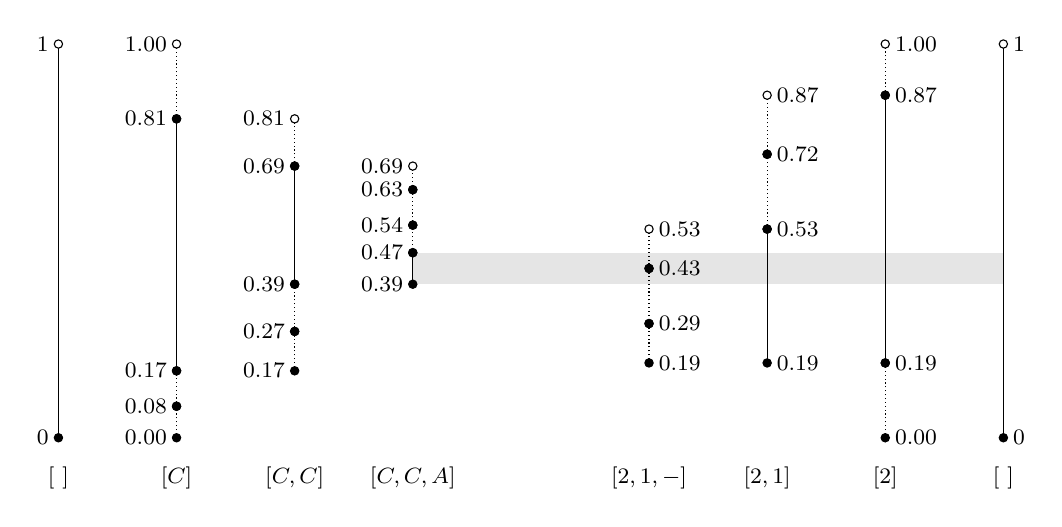
\begin{tikzpicture}[scale=0.05]
		% Final interval range
		\fill [opacity=0.1] (-30,0.39*100) rectangle (120,0.47*100);

		% Input side
		\intervalBothLabels{-120}{0}{100}{0}{1}{solid}{left}
		\node[below] at (-120,-5) {\footnotesize $[~]$};

		\intervalBothLabels{-90}{0}{100}{0.81}{1.00}{densely dotted}{left}
		\intervalBottomLabel{-90}{0}{100}{0.17}{0.81}{solid}{left}
		\intervalBottomLabel{-90}{0}{100}{0.08}{0.17}{densely dotted}{left}
		\intervalBottomLabel{-90}{0}{100}{0.00}{0.08}{densely dotted}{left}
		\node[below] at (-90,-5) {\footnotesize $[C]$};

		\intervalBothLabels{-60}{0}{100}{0.69}{0.81}{densely dotted}{left}
		\intervalBottomLabel{-60}{0}{100}{0.39}{0.69}{solid}{left}
		\intervalBottomLabel{-60}{0}{100}{0.27}{0.39}{densely dotted}{left}
		\intervalBottomLabel{-60}{0}{100}{0.17}{0.27}{densely dotted}{left}
		\node[below] at (-60,-5) {\footnotesize $[C,C]$};

		\intervalBottomLabel{-30}{0}{100}{0.39}{0.47}{solid}{left}
		\intervalBottomLabel{-30}{0}{100}{0.47}{0.54}{densely dotted}{left}
		\intervalBottomLabel{-30}{0}{100}{0.54}{0.63}{densely dotted}{left}
		\intervalBothLabels{-30}{0}{100}{0.63}{0.69}{densely dotted}{left}
		\node[below] at (-30,-5) {\footnotesize $[C,C,A]$};

		% Output side
		\intervalBothLabels{120}{0}{100}{0}{1}{solid}{right}
		\node[below] at (120,-5) {\footnotesize $[~]$};

		\intervalBothLabels{90}{0}{100}{0.87}{1.00}{densely dotted}{right}
		\intervalBottomLabel{90}{0}{100}{0.19}{0.87}{solid}{right}
		\intervalBottomLabel{90}{0}{100}{0.00}{0.19}{densely dotted}{right}
		\node[below] at (90,-5) {\footnotesize $[2]$};

		\intervalBothLabels{60}{0}{100}{0.72}{0.87}{densely dotted}{right}
		\intervalBottomLabel{60}{0}{100}{0.53}{0.72}{densely dotted}{right}
		\intervalBottomLabel{60}{0}{100}{0.19}{0.53}{solid}{right}
		\node[below] at (60,-5) {\footnotesize $[2,1]$};

		\intervalBothLabels{30}{0}{100}{0.43}{0.53}{densely dotted}{right}
		\intervalBottomLabel{30}{0}{100}{0.29}{0.43}{densely dotted}{right}
		\intervalBottomLabel{30}{0}{100}{0.19}{0.29}{densely dotted}{right}
		\node[below] at (30,-5) {\footnotesize $[2,1,-]$};

	\end{tikzpicture}

	\caption{\label{fig:interval_algorithm}Example run of the interval algorithm. On the left, an input sequence $[C,C,A]$ from the source process gets mapped to $[0.39,0.47)$. On the right, this interval allows to generate up to 2 terms of an output sequence from the target process, \ie $[2,1]$, which corresponds to $[0.19,0.53)$. Note that it is not possible to generate more terms of the output sequence, as neither $[0.19,0.29)$ nor $[0.29,0.43)$ nor $[0.43,0.53)$ is a superinterval of $[0.39,0.47)$.}

\end{figure}

\newpage
\section{Statistical natural language models}
\label{sec:snlm}

The notation and theory in section \ref{sec:snlm} is mostly based on \cite{4f11:statistical_language_models, 4f11:smt_systems, coursera:nlp}.

\subsection{Text as the output of a stochastic process}

A string $\mathbf w$ can be regarded as a sequence of $L$ \emph{tokens} $w_1, \dots, w_L$. Tokens are atomic elements of text such as words or punctuation marks:

\begin{equation}
\mathbf w = [ w_1, \dots, w_L ] \equiv w_1^L
\end{equation}

$\mathbf w$ can be regarded as an $L$-dimensional vector of jointly distributed random variables $w_l \in \{1, \dots, V\}$, where $V$ is the number of distinct tokens. According to the chain rule of probability, we can factorise $P(\mathbf w)$ in the following way:

\begin{equation}
\label{eq:exact_string_probability}
P(\mathbf w) = \prod_{l=1}^{L} P( w_l | w_1^{l-1} )
\end{equation}

Even though Eq.~\ref{eq:exact_string_probability} gives a convenient formulation of language as a stochastic process, it is computationally intractable. The conditional probabilities need to be stored in tables. Conditional probability table of just the last token would have $V^L$ entries. With $V \approx 10^6$, this number becomes prohibitively large for even small $L$.

\subsection{$N$-gram language models}

The usual solution is to restrict the size of the context to $N-1$ previous tokens, resulting in an approximate $N$-gram language model:

\begin{equation}
\label{eq:ngram_string_probability}
P(\mathbf w) \approx P_{\text{$N$-gram}}(\mathbf w) \equiv \prod_{l=1}^{L} P( w_l | w_{l-N+1}^{l-1} )
\end{equation}

\subsection{Estimating ML parameters}

Eq.~\ref{eq:ml_conditional_token_probability} gives the ML (maximum likelihood) estimate of conditional probability of $w_l$ in an $N$-gram model. $f(\cdot)$ is the number of occurrences of a particular sequence of tokens in the training dataset.

\begin{equation}
\label{eq:ml_conditional_token_probability}
\hat P( w_l | w_{l-N+1}^{l-1} ) = \frac {f(w_{l-N+1}^l)} {f(w_{l-N+1}^{l-1})}
\end{equation}

A problem with Eq.~\ref{eq:ml_conditional_token_probability} is that most $N$-gram counts will be zero. For example, a $5$-gram model with $V \approx 10^6$ will have $V^L \approx \left( 10^6 \right)^5 = 10^{30}$ distinct $N$-grams. For every possible $5$-gram sequence to occur at least once, the training set would need to consist of $\ge 10^{30}$ tokens. Currently largest available dataset is based on $\approx 3.6 \times 10^{11}$ English words. \cite{googlengrams2011} As a result, a large number of grammatically correct sentences would have zero probability.

\subsection{Limiting database size, discounting and back-off}

A standard way of dealing with this problem is by introducing \emph{discounting} and \emph{back-off} to the model. In addition, $N$-grams with counts below a threshold $C$ are sometimes discarded from the database to conserve storage space. Conditional distribution of the $l$th token becomes:

\begin{equation}
	\label{eq:conditional_token_probability_with_backoff}
	P( w_l | w_{l-N+1}^{l-1} ) =
	\begin{cases}
		d (w_{l-N+1}^l) ~ \frac {f\left(w_{l-N+1}^l \right)} {f\left(w_{l-N+1}^{l-1} \right)} & \text{if $f(w_{l-N+1}^l) \ge C$},\\
		\alpha (w_{l-N+1}^l) ~ P( w_l | w_{l-N+2}^{l-1} ) & \text{otherwise}.
	\end{cases}
\end{equation}

$d(\cdot)$ and $\alpha(\cdot)$ return the discount and back-off weights -- scaling factors used to ensure that Eq.~\ref{eq:conditional_token_probability_with_backoff} is a valid \pmf. Intuitively, they reduce the mass assigned to observed $N$-grams to accommodate for estimates of order $N-1$ and lower. $d(\cdot)$ and $\alpha(\cdot)$ are hard to choose or compute -- there exist many different schemes motivated by linguistics and statistics. Examples include Good-Turing smoothing,\cite{good1953} Kneser-Ney smoothing,\cite{kneserney1995} or stupid back-off.\cite{brants2007} All exhibit various levels of complexity and for example the last one does not even return a valid \pmf.

\section{Processing and storing $N$-gram counts}

\subsection{Sources of natural language statistical data}

Make a table comparing COCA and Google Books $N$-grams. Indicate that I've chosen Google Books $N$-grams because they are free and have a higher order.

\subsection{Google Books $N$-grams format}

\subsection{Normalising tokens}

\subsubsection{Discarding $N$-grams containing digits}

The Google Books $N$-grams database is based on many books, some of which include data tables. As a result, they contain a large number of $N$-grams consisting of just numbers and punctuation marks. Randomly generated text would sometimes include long sequences of those. I decided to discard $N$-grams containing digits to avoid such possibility and focus on generating natural language. The only trade-off is that dates that use digits to write days of the month will not longer be a part of the language.

\subsubsection{Normalising tokens using the \texttt{unidecode} package}

\subsection{Exploding tokens by punctuation}

Use the \emph{it's} example.

\subsubsection{Induced exploded $N$-gram counts}

Describe algorithm to calculate induced lower-order counts after exploding $N$-grams.

\subsection{Ensuring counts consistency}

\subsection{Sentence delimiters}

\subsection{BinDB file format}

\section{Language model}

\subsection{Requirements}
\label{eq:lm_requirements}

Language model fit for steganographic application using the interval algorithm needs to satisfy certain requirements:

\begin{enumerate}
  \item \label{lm_req:non_zero_probability} Every sequence of tokens has non-zero probability.
  \item \label{lm_req:contiguous_probability} Every token extending a sequence is assigned a contiguous probability region.
  \item \label{lm_req:hidden_symbols} Formatted sequence of tokens uniquely identifies the tokens.
\end{enumerate}

Requirement \ref{lm_req:non_zero_probability} warrants the use of back-off. Consider the counts from Tab.~\ref{tab:the_esteem_of_many_CONT} and Tab.~\ref{tab:the_esteem_of_many}. In the 5-gram model, only 5 tokens are explicitly allowed to follow \emph{the esteem of many} and their total count is 542. If we used the ML model from Eq.~\ref{eq:ml_conditional_token_probability} to calculate their probabilities, we would assign zero probability to all tokens other than those in column $w_5$ of Tab.~\ref{tab:the_esteem_of_many_CONT}. Thus, we would account for only $\frac {542} {1146} \approx 0.47$ of the probability mass and also discard the vast majority of tokens. The former problem can be mitigated by upscaling the probabilities, but the latter has no solution other than back-off.

\begin{table}[h]
	\centering
	\begin{tabular}{c | *{5}{| c} || c}
	index & $w_1$ & $w_2$ & $w_3$ & $w_4$ & $w_5$ & $f(w_1^5)$ \\
	\hline
	\num{400000787} & the & esteem & of & many & , & 143 \\
	\num{400000788} & the & esteem & of & many & . & 56 \\
	\num{400000789} & the & esteem & of & many & friends & 66 \\
	\num{400000790} & the & esteem & of & many & of & 237 \\
	\num{400000791} & the & esteem & of & many & who & 40
	\end{tabular}
	\caption{\label{tab:the_esteem_of_many_CONT}Counts of all 5-grams beginning with \emph{the esteem of many}.}
\end{table}

\begin{table}[h]
	\centering
	\begin{tabular}{c | *{4}{| c} || c}
	index & $w_1$ & $w_2$ & $w_3$ & $w_4$ & $f(w_1^4)$ \\
	\hline
	\num{456820272} & the & esteem & of & many & 1146
	\end{tabular}
	\caption{\label{tab:the_esteem_of_many}Count of \emph{the esteem of many} 4-gram.}
\end{table}

Requirement \ref{lm_req:hidden_symbols} greatly complicates the language model. If arithmetic coding is only used to compress text, it is possible to augment the sequence during encoding by inserting \emph{explicit} back-off symbols. Their purpose is to indicate during decoding that the next token's probability is to be evaluated using a lower-order model. But in a steganographic scenario, the usage of a back-off symbol would compromise innocuousness of the system. Therefore an \emph{implicit} back-off scheme is needed.

The problem with implicit back-off and using Eq.~\ref{eq:conditional_token_probability_with_backoff} \emph{exactly} is that if a token has non-zero probability in \eg a 5-gram model, by counts consistency it is also included in all lower-order models. As a result, there are 5 separate probability regions corresponding to it -- one in each back-off level (\ie in models from 5-gram to 1-gram). These intervals will not be contiguous and requirement \ref{lm_req:contiguous_probability} will be violated.

\subsection{Back-off tree}

Fig.~\ref{fig:backoff_tree} shows how to construct a \emph{back-off tree} where each token is represented by a single leaf. Each leaf corresponds to a contiguous, non-zero interval. The set of all leaf intervals partitions $[0,1)$. As a result, they tree can be interpreted as giving a \pmf over all tokens that satisfies all requirements from the previous section.

% Define a new tikz style for drawing vertices
\newlength{\vertexSize}
\setlength{\vertexSize}{10 pt}
\tikzset{
    vertex/.style={
        circle,
        draw,
        inner sep = 0pt,
        minimum width = \vertexSize
    }
}

% Define macros for drawing vertices

%	rootVertex: vertex without any edges
%
%	(#1,#2)	- coordinates
\newcommand{\rootVertex}[2] {
	\node [vertex,fill=black!0] at (#1,#2) {};
}

% 	connectedVertex: vertex connected to a previous vertex
%
%	(#1,#2)	- previous vertex coordinates
%	(#3,#4)	- coordinates
%	#5		- bend
%	#6		- label
\newcommand{\backoff}[6] {
	\draw [shorten >= 0.5*(\vertexSize+\pgflinewidth), shorten <= 0.5*(\vertexSize+\pgflinewidth), ->] (#1,#2) to [bend #5=12.5] (#3,#4);
	\node [vertex,fill=black!10] at (#3,#4) {\tiny #6};
}

% 	connectedLeaf: leaf vertex connected to a previous vertex
%
%	(#1,#2)	- previous vertex coordinates
%	(#3,#4)	- coordinates
%	#5		- bend
%	#6		- label
\newcommand{\leaf}[6] {
	\draw [shorten >= 0.5*(\vertexSize+\pgflinewidth), shorten <= 0.5*(\vertexSize+\pgflinewidth), ->] (#1,#2) to [bend #5=12.5] (#3,#4);
	\node [vertex,fill=black!0] at (#3,#4) {\tiny #6};
}

\begin{figure}[h]
\centering
\begin{tikzpicture}[scale=0.5]

	% The context  words from w_A to w_D
	\rootVertex{6}{9.5}
	\node[left] at (5.5,9.5) {\scriptsize $w_{l-4}^{l-1}$};

	% First level word leaves
	\leaf{6}{9.5}{9}{-1}{right}{3}
	\leaf{6}{9.5}{9}{0}{right}{7}
	\leaf{6}{9.5}{9}{1}{right}{17}

	% First level backoff node
	\backoff{6}{9.5}{9}{11}{left}{$b_1$}


	% Second level word leaves
	\leaf{9}{11}{12}{2}{right}{4}
	\leaf{9}{11}{12}{3}{right}{13}
	\leaf{9}{11}{12}{4}{right}{15}
	\leaf{9}{11}{12}{5}{right}{20}

	% Second level backoff node
	\backoff{9}{11}{12}{13}{left}{$b_2$}


	% Third level word leaves
	\leaf{12}{13}{15}{6}{right}{1}
	\leaf{12}{13}{15}{7}{right}{16}

	% Third level backoff node
	\backoff{12}{13}{15}{14}{left}{$b_3$}


	% Fourth level word leaves
	\leaf{15}{14}{18}{8}{right}{6}
	\leaf{15}{14}{18}{9}{right}{9}
	\leaf{15}{14}{18}{10}{right}{10}
	\leaf{15}{14}{18}{11}{right}{12}
	\leaf{15}{14}{18}{12}{right}{14}

	% Fourth level backoff node
	\backoff{15}{14}{18}{16.5}{left}{$b_4$}


	% Fifth level word leaves
	\leaf{18}{16.5}{21}{13}{right}{2}
	\leaf{18}{16.5}{21}{14}{right}{5}
	\leaf{18}{16.5}{21}{15}{right}{8}
	\leaf{18}{16.5}{21}{16}{right}{11}
	\leaf{18}{16.5}{21}{17}{left}{18}
	\leaf{18}{16.5}{21}{18}{left}{19}
	\leaf{18}{16.5}{21}{19}{left}{21}
	\leaf{18}{16.5}{21}{20}{left}{22}

	% Draw the intervals and the dashed line showing correspondence to leaves
	\draw[dashed] [shorten >= 1.5 pt] (9,20.5) -- (23,20.5);
	\draw[solid] [i] (23,12.5) -- (23,20.5);
	\draw[dashed] (18,12.5) -- (23,12.5);
	\draw[solid] [i] (23,7.5) -- (23,12.5);
	\draw[dashed] (15,7.5) -- (23,7.5);
	\draw[solid] [i] (23,5.5) -- (23,7.5);
	\draw[dashed] (12,5.5) -- (23,5.5);
	\draw[solid] [i] (23,1.5) -- (23,5.5);
	\draw[dashed] (9,1.5) -- (23,1.5);
	\draw[solid] [i] (23,-1.5) -- (23,1.5);
	\draw[dashed] (9,-1.5) -- (23,-1.5);

	% Draw thin dotted lines showing token correspondence to intervals
	\draw[dotted, thin] (9,-0.5) -- (23,-0.5);
	\draw[dotted, thin] (9,0.5) -- (23,0.5);

	\draw[dotted, thin] (12,2.5) -- (23,2.5);
	\draw[dotted, thin] (12,3.5) -- (23,3.5);
	\draw[dotted, thin] (12,4.5) -- (23,4.5);

	\draw[dotted, thin] (15,6.5) -- (23,6.5);

	\draw[dotted, thin] (18,8.5) -- (23,8.5);
	\draw[dotted, thin] (18,9.5) -- (23,9.5);
	\draw[dotted, thin] (18,10.5) -- (23,10.5);
	\draw[dotted, thin] (18,11.5) -- (23,11.5);

	\draw[dotted, thin] (21,13.5) -- (23,13.5);
	\draw[dotted, thin] (21,14.5) -- (23,14.5);
	\draw[dotted, thin] (21,15.5) -- (23,15.5);
	\draw[dotted, thin] (21,16.5) -- (23,16.5);
	\draw[dotted, thin] (21,17.5) -- (23,17.5);
	\draw[dotted, thin] (21,18.5) -- (23,18.5);
	\draw[dotted, thin] (21,19.5) -- (23,19.5);

	% Label the interval ends
	\node[above] at (23,20.5) {\footnotesize 1};
	\node[below] at (23,-1.5) {\footnotesize 0};

	% Define sets of leaves in a certain level (with braces)
	\draw [decorate,decoration={brace,amplitude=5pt,raise=5pt,mirror}] (23,-1.4) -- (23,1.4) node [midway,right,xshift=10pt] {\scriptsize $\mathcal W_1 = \left\{ w_l : f(w_{l-4}^l) \ge C \right\}$ };
	\draw [decorate,decoration={brace,amplitude=5pt,raise=5pt,mirror}] (23,1.6) -- (23,5.4) node [midway,right,xshift=10pt] {\scriptsize $\mathcal W_2 = \left\{ w_l : f(w_{l-3}^l) \ge C \land f(w_{l-4}^l) < C \right\}$ };
	\draw [decorate,decoration={brace,amplitude=5pt,raise=5pt,mirror}] (23,5.6) -- (23,7.4) node [midway,right,xshift=10pt] {\scriptsize $\mathcal W_3 = \left\{ w_l : f(w_{l-2}^l) \ge C \land f(w_{l-3}^l) < C \right\}$ };
	\draw [decorate,decoration={brace,amplitude=5pt,raise=5pt,mirror}] (23,7.6) -- (23,12.4) node [midway,right,xshift=10pt] {\scriptsize $\mathcal W_4 = \left\{ w_l : f(w_{l-1}^l) \ge C \land f(w_{l-2}^l) < C \right\}$ };
	\draw [decorate,decoration={brace,amplitude=5pt,raise=5pt,mirror}] (23,12.6) -- (23,20.4) node [midway,right,xshift=10pt] {\scriptsize $\mathcal W_5 = \left\{ w_l : f(w_l) \ge C \land f(w_{l-1}^l) < C \right\}$ };

%	% Define sets of leaves in a certain level
%	\node [right,xshift=10pt] at (23,0) {\scriptsize $\mathcal W_1 = \left\{ w_l : f(w_{l-4}^l) \ge C \right\}$ };
%	\node [right,xshift=10pt] at (23,3.5) {\scriptsize $\mathcal W_2 = \left\{ w_l : f(w_{l-3}^l) \ge C \land f(w_{l-4}^l) < C \right\}$ };
%	\node [right,xshift=10pt] at (23,6.5) {\scriptsize $\mathcal W_3 = \left\{ w_l : f(w_{l-2}^l) \ge C \land f(w_{l-3}^l) < C \right\}$ };
%	\node [right,xshift=10pt] at (23,10) {\scriptsize $\mathcal W_4 = \left\{ w_l : f(w_{l-1}^l) \ge C \land f(w_{l-2}^l) < C \right\}$ };
%	\node [right,xshift=10pt] at (23,16.5) {\scriptsize $\mathcal W_5 = \left\{ w_l : f(w_l) \ge C \land f(w_{l-1}^l) < C \right\}$ };

	% Label the levels
	\node[below] at (9,-2.5) {\footnotesize level 1};
	\node[below] at (12,-2.5) {\footnotesize level 2};
	\node[below] at (15,-2.5) {\footnotesize level 3};
	\node[below] at (18,-2.5) {\footnotesize level 4};
	\node[below] at (21,-2.5) {\footnotesize level 5};

	% Label the intervals in level 1
%	\draw [decorate,decoration={brace,amplitude=5pt,raise=5pt,mirror}] (35,-1.5) -- (35,1.5) node [midway,right,xshift=10pt] {\scriptsize $\frac {\sum_{w_l \in \mathcal W_1} f(w_{l-4}^l)} {b_1 + \sum_{w_l \in \mathcal W_1} f(w_{l-4}^l)}$};
%	\draw [decorate,decoration={brace,amplitude=5pt,raise=5pt,mirror}] (35,1.5) -- (35,20.5) node [midway,right,xshift=10pt] {\scriptsize $\frac {b_1} {b_1 + \sum_{w_l \in \mathcal W_1} f(w_{l-4}^l)}$};

\end{tikzpicture}
\caption{\label{fig:backoff_tree}Example back-off tree for context $w_{l-4}^{l-1}$, \ie with $N=5$. Leaf labels $w_l \in \left\{ 1, \dots, V \right\}$ correspond to token indices. In this example $V=22$.}
\end{figure}

A different back-off tree is defined for each context $w_{l-N+1}^{l-1}$. The first level contains leaf nodes corresponding to tokens that belong to the set $\mathcal W_1 = \left\{ w_l : f(w_{l-N+1}^l) \ge C \right\}$ and a single back-off parent node $b_1$. Each node is assigned a count $c(\cdot)$. For the leaves the count is simply $c(w_l) = f(w_{l-N+1}^l)$. Calculating the back-off pseudo-count $c(b_1)$ is covered in the next section. Nodes are arranged in the following way: leaves in order of increasing index followed by the back-off node. They partition $[0,1)$ into corresponding intervals $v(\cdot)$ with size proportional to the node count.

Subsequent levels of depth $d \in \left\{ 2, \dots, N \right\}$ are constructed analogously. One difference is that the set of leaf nodes is $\mathcal W_d = \left\{ w_l : f(w_{l-N+d}^l) \ge C \land f(w_{l-N+d-1}^l) < C \right\}$. Nodes do not partition $[0,1)$, but $v(b_{d-1})$ -- interval assigned to the back-off node in the previous level. There is also no back-off node in the last level.

Intuitively, level 1 tokens are the ones that give non-zero probability in an ML language model of order $N$. Level 2 tokens give non-zero probability in an ML model of order $N-1$, but do not include tokens from level 1. Tokens in levels of depth $d \ge 3$ are chosen analogously and exclude tokens from \emph{all} previous levels. By counts consistency it suffices to check that $f(w_{l-N+(d-1)}^l) \ge C$ to exclude a token from level $d$. If it satisfies the inequality, it must have appeared in \emph{some} previous level: $d-1$ or earlier.

Sizes of intervals $v(w_l)$ are proportional to the ML estimate $\hat P(w_l | w_{l-N'+1}^{l-1})$ for highest $N' \le N$ that gives a non-zero value. The constant of proportionally is different for each level of the back-off tree and depends on the back-off pseudo-counts $c(b_1), \dots, c(b_{N-1})$.

\subsection{$\beta-\gamma$ algorithm for calculating back-off pseudo-counts}

The value $c(b_d)$ needs to reflect the probability that a not explicitly allowed token follows the context. I propose the following algorithm for assigning back-off pseudo-count in the first level of back-off tree:
%
\begin{align}
\label{eq:total_probability_mass} m &= f(w_{l-N+1}^{l-1}) \\
\label{eq:backoff_pseudocount_level1} c(b_1) &= \ceil*{ \beta \bracket*{ m - \sum_{w_l \in \mathcal W_1} f(w_{l-N+1}^l) } + \gamma ~ m }
\end{align}

Parameter $\beta$ controls what proportion of the \emph{leftover probability mass} is used to account for the event of a back-off. $\gamma$ controls how much of the \emph{total probability mass} is added to account for back-off. To illustrate using the example from Section~\ref{eq:lm_requirements}, the total probability mass is $m = 1146$ and the leftover probability mass is $1146-542=604$.

Dealing with excluded tokens in a deeper level $d$ of the back-off tree is not difficult. It suffices to restate the total probability mass as $\overline m$ to remove counts of excluded tokens:

\begin{equation}
\label{eq:adjusted_total_probability_mass}
\overline m = f(w_{l-N+d}^{l-1}) - \sum_{w_l \in \mathcal W_1 \cup \dots \cup \mathcal W_{d-1}} f(w_{l-N+d}^l)
\end{equation}

Then the calculation from Eq.~\ref{eq:backoff_pseudocount_level1} can be repeated in an analogous way.

\begin{equation}
\label{eq:backoff_pseudocount_deep_levels}
c(b_d) = \ceil*{ \beta \bracket*{ \overline m - \sum_{w_l \in \mathcal W_d} f(w_{l-N+d}^l) } + \gamma ~ \overline m }
\end{equation}

The only special case to consider is when $m=0$ or $\overline m = 0$. This can simply occur if the context was observed in the training dataset fewer than $C$ times, but also in more subtle situations.\footnote{If all tokens in a level are excluded \emph{and} the context count $f(w_{l-N+d}^{l-1})$ is equal to the sum of excluded counts $f(w_{l-N+d}^l)$ then $\overline m$ will be 0. This happens if the context was observed in the training set only followed by the excluded tokens.} Back-off pseudo-count would be then 0, but the back-off node would be the only node in its level anyway. It can be arbitrarily given a count of 1, or just assigned the full interval corresponding to its level regardless of the pseudo-count.

\newpage
\section{Detailed description of the stegosystem}

Lorem ipsum.

\subsection{Source -- plaintext concatenated with randomness}

\subsection{Target -- English language model}

\subsection{Storing length of plaintext}

\subsubsection{Universal coding of plaintext length}

\subsubsection{EOF symbol}

\subsection{Sufficient length of the output interval}

\subsection{Secrecy}

\newpage
\section{Implementation}

Lorem ipsum.

\newpage
\section{Security vulnerabilities}

Lorem ipsum.

\subsection{Telling stegotext from covertext}

\subsubsection{Plaintext length declaration incompatible with interval size}

If the plaintext length declaration is longer than the maximum length of plaintext that can be recovered from the potential stegotext, we know the message was covertext.

Conversely -- how often does a compatible length declaration indicate stegotext? If almost always, then the system is flawed.

\newpage
\section{Theoretical considerations}

Lorem ipsum.

\subsection{Rate of the system}

\subsection{Entropy of the language model and its effect on stegotext length}

Use the bounds from Han \& Hoshi's paper.

\newpage
\section{Interesting questions}

Lorem ipsum.

\subsection{How many bits of information stored per word, sentence, tweet?}

\subsubsection{Dependence on the entropy of the language model}

\newpage
\footnotesize
\bibliographystyle{unsrt}
\bibliography{../bibliography}

\newpage
\appendix

\section{First appendix}

\end{document}